\chapter{Game Design Document}\label{ap:gdd}
\section{Visão geral essencial}
%A principal função da primeira seção do documento é fazer com que qualquer pessoa se familiarize rapidamente com a idéia do jogo, o que o fará se destacar e --- ter boa jogabilidade.

Em ``crimechanics'' o jogador deve arquitetar diversos roubos em uma cidade controlando uma gangue de engenheiros, cada um com suas habilidades específicas. O jogador deve fazer o reconhecimento dos alvos, conversar com personagens para coletar informações sobre o alvo e comprar itens para sua equipe. No entanto, é preciso ter cautela, a polícia já foi avisada e fará o possível para evitar os roubos.

\subsection{Resumo}
%O resumo é uma síntese de toda a experiência do jogo.

A interação com o jogo se dá principalmente  por meio de diálogos e menus. Assim o jogador compra itens, estuda a segurança dos lugares que pretende roubar, gerencia a equipe a participar de cada investida e também os dividendos dos participantes.

\subsection{Aspectos fundamentais}
%O objetivo desta seção é extrair componetes fundamentais do jogo que constituirão a trama central para a experiência e a diversão do jogador.

O jogo narra a história de um grupo de engenheiros, cujo líder é controlado pelo jogador, que planejam subverter a ordem do poder local. A cidade é uma cidade planejada pelos próprios engenheiros, para ser um ambiente sustentável e um modelo de igualdade social. Acontece que um dos maiores investidores do projeto, o dr. Pinheirótopos, mudou as regras do jogo perto do fim, e, mostrando-se um prefeito despótico ao assumir o cargo, proibiu o exercício de engenharia no perímetro da cidade. Além disso, transformou-a num paraíso para abastados, decidindo pelo número de dígitos no saldo da conta bancária os cidadãos que teriam direito a viver em \nomeCidade.

Com o intuito de esvaziar a cidade, e esvaziar o poder do autoproclamado prefeito Pinheirótopos, o grupo de projetistas da cidade se organiza clandestinamente e passa a planejar roubos, desacreditando a segurança que eles mesmos haviam concebido para a cidade.


Sem emprego, e revoltados com o rumo dos acontecimentos, o grupo ilegal de engenheiros se forma: os \nomeGrupo{} se preparam para uma batalha épica contra o prefeito.

\subsection{Golden nuggets}
Na concepção da inteligência artificial do jogo foi empregada a arquitetura BDI para agentes, com a finalidade de torná-los mais realistas e adaptáveis do que simples máquinas de estados. Com isso, a interação do usuário com os \npc{}s será muito mais rica, pois o rumo de um diálogo passa a ser mais imprevisível.

\section{Contexto do jogo}
\subsection{História}

Há muitos anos um homem, doutor Pinheirótopos convenceu diversos colegas, todos eles engenheiros, a investirem muito tempo e muito dinheiro em um projeto para fundar uma cidade onde pessoas mais pobres teriam acesso a educação e saúde e poderiam levar uma vida digna. Os engenheiros perderam muitas noites de sono desenhando plantas de edifícios e desenvolvendo sistemas para melhorar a qualidade de vida das pessoas que lá habitariam.
No entanto, Pinheirótopos deu um golpe, elegeu-se prefeito da cidade, e mostrou suas verdadeiras intenções: aumentou impostos, criando com isso uma barreira para justo aqueles para quem a cidade havia sido projetada; os cidadãos que não conseguiam pagar a vida na cidade foram deslocados para periferias e separados da cidade pela polícia.

Pinheirótopos ficou muito rico e transformou a pequena cidade em um pequeno império, em que apenas pessoas selecionadas  por ele poderiam morar. Deu preferência a amigos, conhecidos e àqueles que sabiam agradá-lo. Detém total controle da cidade, afinal (sic) fora projetada por engenheiros, devido a um avançado sistema de segurança, com câmeras espalhadas pelas ruas monitorando a movimentação na cidade 24 horas por dia, e um sistema de alarmes em todos os edifícios que se comunica diretamente com a sede da polícia. Além disso, Pinheirótopos proibiu o emprego de engenheiros na cidade. Esta lei absurda nasceu de uma rivalidade universitária de sua juventude, que o prefeito havia ocultado por longos anos.

Na periferia da cidade, os engenheiros que construíram este sonho se uniram e agora estão dispostos a recuperar a cidade das mãos deste poderoso e inescrupuloso homem. Para isso, a solução encontrada foi deixar a população seleta de Pinheirótopos insatisfeita com o lugar e seu regente. Os engenheiros se organizaram e montaram uma “gangue”, os \nomeGrupo{}, que roubará os melhores estabelecimentos da cidade para enfraquecer a economia da cidade e mostrar que ninguém está seguro e nem protegido como sempre garantiu Pinheirótopos.

%\subsection{Eventos anteriores}
%Esta seção explica o contexto da história do jogo. Dependendo da simplicidade do projeto %pode ser vazia.


\subsection{Principais jogadores}
%Se no projeto do jogo os personagens forem elementos-chave, nesta seção devem ser apresentados e explicados os principais personagens do jogo.

O jogador controla um personagem que gerencia as atividades dos \nomeGrupo. Ele é um engenheiro, mas especialidade é desconhecida, e seu papel no grupo é coordenar, muito mais do que executar os roubos propriamente ditos.

\section{Objetos essenciais do jogo}

\subsection{Personagens}
%Esta seção descreve os personagens do jogo, desde os principais personagens envolvidos na histório da jogo aos \npc{}s aliados ou inimigos menos importantes.


Os personagens do jogo estão divididos em três classes: civis, policiais e capangas.

Os civis são agentes que estão espalhados nos níveis do jogo, o jogador pode iniciar diálogos com qualquer civil presente e dependendo do desenrolar da conversa pode conseguir informações sobre determinados alvos ou mesmo desbloquear itens, que passam a poder ser comprados (ou até mesmo conquistados) e usados nos roubos.

Os policiais são agentes espalhados nos níveis do jogo que observam as ações ao seu redor e reportam à central da polícia qualquer atividade que considerem suspeita. Além disso, podem efetuar prisões de capangas. O jogador também pode iniciar diálogos com um policial e num caso de sucesso pode tentar suborná-lo e descobrir informações importantes sobre o processo de investigação da polícia. Além disso, existem agentes policiais que são ocultos ao jogador, estes agentes são responsáveis pelo processamento das informações no blackboard.

Os capangas que compõem a gangue também são agentes, a maior diferença em relação aos outros tipos de agentes é que todos os capangas possuem uma mesma lista de habilidades. A especialidade de cada um (elétrico, computação, produção, químico, mecânico ou civil) influencia diretamente em seu desempenho em tarefas específicas.
Todos os personagens são agentes criados utilizando a arquitetura BDI.

\subsubsection{Lista de habilidades}
\begin{table}\footnotesize
\begin{tabular}{ccccccc}
& computação & civil & elétrico & mecânico & produção & químico \\
\hline
invadir sistema & 7&2&4&2&2&2\\
reconhecimento de segurança & 3&7&4&4&2&2\\
danificar infra-estrutura &3&7&5&4&2&3\\
desligar aparelhos &6&4&7&3&2&2\\
falsificar crachá &3&4&7&2&6&2\\
arrombar &3&5&4&7&2&4\\
carisma &3&4&2&4&8&5\\
explodir &3&5&3&4&2&7\\
arma química &3&1&1&1&2&7\\
força &4&5&2&7&6&5\\
pontaria &5&5&5&6&5&5\\
\hline
\end{tabular}
\caption{Matriz de habilidades dos capangas.}\label{tab:habilidadesCapang}
\end{table}


\subsection{Características comuns dos agentes}
Todos os agentes possuem ao menos duas características em comum, sua \emph{personalidade} e  \emph{estados psicológicos}. Estas características são importantes pois é graças a elas que os agentes conseguem deliberar durante um diálogo. Elas influenciam diretamente nas ações e respostas do mesmo.

É válido ressaltar a difernça conceitual entre ambas as características. O estado psicológico de um agente pode ser visto como o análogo do estado de um autômato. A principal diferença entre ambos é que as transições de estado psicológico dependem do contexto percebido pelo agente. Além disso, fixados um contexto e uma tendência a alteração do estado psicológico, situação mais detalhada posteriormente nesta seção, o próximo estado psicológico dependerá também da personalidade do agente, que reflete, de certo modo, como o agente reage a estímulos. Note-se que a personalidade não é algo fixo, embora altere-se raramente. Retomando a analogia com autômatos, e expandindo-a de certa forma, é como se personalidades distintas fossem conjuntos de estados próximos entre si, com grande probabilidade de serem visitados em seguida para a maior parte das cadeias. Assim, é improvável que um agente mude de personalidade, enquanto, por outro lado, é provável que vários estados psicológicos associados a uma mesma personalidade sejam visitados durante a operação do agente.


Além disso, existem \emph{estímulos}, que são gerados conforme o jogador opta por determinadas falas durante um diálogo com um agente. O agente recebe então estes estímulos, e varia seu estado psicológico ou até mesmo sua personalidade de acordo com os estímulos recebidos.

\subsubsection{Tipos de personalidades}
Abaixo são listados os possíveis estados psicológicos em que um agente pode estar durante um diálogo. Cada estado psicológico influencia  as decisões do agente de alguma forma.
%-->> Listar as personalidades
\begin{itemize}
\item rabugento
\item simpático
\item educado
\item grosseiro
\item apressado
\end{itemize}

\subsubsection{Tipos de estados psicológicos}
Abaixo são listados os possíveis estados psicológicos em que um agente pode estar durante um diálogo. Cada estado psicológico influencia  as decisões do agente de alguma forma.
%-->> Listar os estados psicológicos
\begin{itemize}
\item feliz
\item zangado
\item apreensivo
\item lisonjeado
\item compreensivo
\end{itemize}

\subsubsection{Tipos de estímulos}
Abaixo são listados os estímulos que são enviados a um agente durante um diálogo conforme as falas que o jogador seleciona.
%Listar os estímulos
\begin{itemize}
\item oferece-propina (Estímulo exclusivo aos agentes policiais)
\item fala-amigavel
\item elogio
\item insulto
\item fala-timida
\item inquisitivo
\item suspeito
\item inquestionavel
\end{itemize}

\subsubsection{Tipos de estado (Policial)}
No caso dos agentes policiais existe uma variável \emph{conduta} que é determinante no caso de um suborno, podendo assumir apenas dois valores.
\begin{itemize}
\item lisonjeado
\item compreensivo
\end{itemize}

\subsubsection{Tipos de reações}
Durante um diálogo, quando for possível aos \npc{}s selecionar mais de uma opção de resposta, eles vão receber os estímulos e em função de sua personalidade e estado psicológico escolherão um tipo de reação que define qual a fala que o agente deseja falar.
\begin{itemize}
\item aceita-propina
\item rejeita-propina
\item insultar
\item elogiar
\item agradecer
\end{itemize}


\subsection{Armas}
O sucesso de um roubo depende muito das habilidades de cada capanga da gangue. As habilidades são iguais para todos os capangas (ou seja, não existem ``classes'' diferentes), o que varia é o quão bem desenvolvida é a habilidade em cada capanga. Além disso, existem itens que o jogador pode comprar e equipar seus capangas com a finalidade de aumentar o nível de habilidades específicas.

\subsubsection{Lista de itens}

Segue uma lista dos itens disponíveis para compra no mercado do jogo (``Lojas Tem’’, tudo o que você precisa!''), em que são discriminadas pequenas descrições que serão apresentadas ao jogador.

\begin{description}
\item[arma] Use com responsabilidade! [é necessário fazer registro! (ou não)]
\item[picareta] Tool-kit casa dos seus sonhos.
\item[dormeflex] Remédio para adormecer (mamíferos em geral)
\item[bife] O prato favorito dos cães.
\item[chave de fenda] Imprescindível!
\item[maçarico] Tool-kit casa dos seus sonhos. Sabendo usar, abre até cofres!
\item[ácido sulfúrico] Nas mãos certas dissolve tudo!
\item[tnt] Ideal para demolições bem barulhentas
\item[terno] Todo mundo fica bem de terno!
\item[cosméticos] Para embelezar!
\item[alicate] Tool-kit casa dos seus sonhos.
\item[pda] Veja seu email ou jogue tetris na fila de espera!
\item[máscara de carnaval] Ninguém vai te reconhecer!
\item[fralda] Deixe seu bebê sequinho e confortável!
\item[fantasia de ladrão] Máscara, luvas e tudo o mais que um ladrão precisa! (para uma festa!)
\item[Rainequem] Para animar qualquer festa! Beba geladinha!
\item[corta-vidro] Tool-kit casa dos seus sonhos.
\item[hp] Não saia de casa sem a sua.
\item[jornal] Palavras cruzadas!
\end{description}

\subsection{Estruturas}
O jogo acontece em uma cidade fictícia onde existem três tipos estruturas, os alvos que são estabelecimentos que o jogador tentará roubar, o quartel general (chamado de ``oficina mecanica’’) que apresenta a interface de controle da equipe para o jogador poder arquitetar os roubos e o mercado onde o jogador pode comprar itens para equipar seus capangas.
Na tela de apresentação é mostrado um mapa da cidade, numa visão superficial onde o jogador pode clicar em cada estrutura para analisar as opções disponíveis em cada caso.
No caso dos alvos, todos possuem uma variável (interna) chamada \emph{nível de segurança} que representa o nível de atenção que a polícia dedica a um determinado alvo, quanto maior o valor da variável maior será o esquema de segurança associado ao lugar e, consequentemente, menores são as chances de um roubo ser bem sucedido.

%-->> Listar os alvos
Os possíveis alvos são os seguintes:
\begin{itemize}
\item loja de importados,
\item loja de carros,
\item banco, e
\item joalheria.
\end{itemize}

%\subsection{Objetos} (NÃO HÁ)

\section{Conflitos e soluções}
No jogo proposto, o adversário do jogador é a polícia. A polícia fará o possível para prender os capangas do jogador e frustrar as tentativas de roubo. A prisão é decretada se o nível de suspeita de um capanga, que é uma variável oculta que a polícia atribui a cada capanga, chegar a um nível muito elevado. Além disso, a polícia pode aumentar o nível de segurança de um alvo se, segundo a inteligência da polícia (blackboard), existirem chances do local ser um alvo.

O jogador deve tomar cuidado para não perder capangas, evitando fazer atividades supeitas como reconhecimento e diálogos nos quais o \npc{} com quem esteja conversando se ofenda e tome uma atitude que possa chamar a atenção do policial no cenário.
Um capanga preso fica indisponível, o jogo termina se o jogador perder todos os seus capangas.

Além disso, o jogador pode tentar subornar um policial para descobrir informações sobre os níveis de segurança dos alvos e os níveis de suspeita dos capangas, mundi dessas informações o jogador pode alterar sua estratégia, utilizar outro capanga ou roubar outro alvo. É importante lembrar que um suborno mau sucedido implica na prisão direta do capanga em uso.

\section{Inteligência Artificial}
O uso da arquitetura BDI tem como objetivo melhorar a experiência do jogador, principalmente durante os diálogos.

No jogo em questão todos os \npc{}s são agentes modelados através da arquitetura BDI. Os agentes foram modelados de forma que conforme um diálogo acontece, suas respostas variam de acordo com seu estado interno, e este, por sua vez, varia de acordo com estímulos que são enviados pelo jogador de forma subliminar através dos diálogos, por exemplo, se um agente tem uma personalidade simpática e um estado psicológico feliz e recebe como estímulo do jogador um elogio, seu estado psicológico passa a ser \emph{lisonjeado} e ele provavelmente optará por uma resposta que expresse sua gratidão.

Além disso, foi utilizada uma técnica conhecida como blackboard de solução de problemas de forma cooperativa que é utilizada por agentes da polícia, ocultos ao jogador, que através desta processam informações enviadas pelos agentes policiais das fases.

Um agente policial nota alguma atividade suspeita e envia essa informação para uma base de conhecimento a qual os agentes ocultos possuem acesso. Estes agentes ocultos processam essa informação e podem (ou não) enviar a todos os agentes policiais alguma nova ação que deve ser realizada, tal ação é passada a todos os agentes policiais como um objetivo na arquitetura BDI.
A figura \ref{blackboard_policia} apresenta de forma visual a estrutura descrita acima.
\begin{figure}
\centering
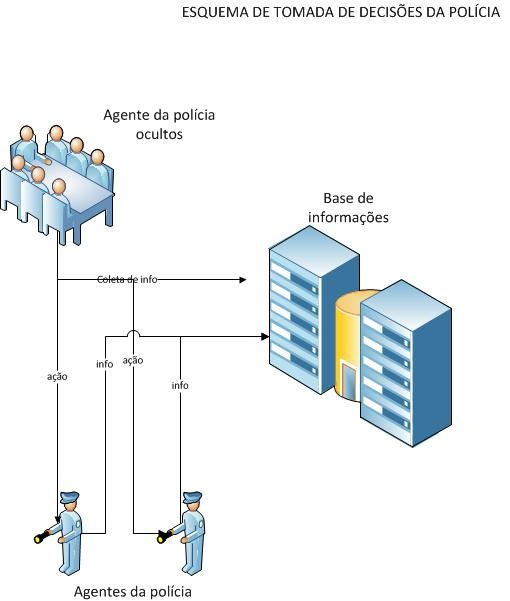
\includegraphics [height=10cm]{figuras/blackboard_policia.jpg}
\caption{Esquema do blackboard no jogo}
\label{blackboard_policia}
\end{figure}

\section{Fluxo do jogo}\label{fluxo-jogo}
%basicamente o guia dos programadores, artistas, designers de níveis e de missões. Aqui devem ser detalhados todos os aspectos de como o jogo funcionará
%De longe a mais longa!

Ao iniciar o jogo, é apresentada uma tela com as opções \emph{novo jogo}, \emph{carregar jogo salvo} ou \emph{sair}. O jogador pode selecionar qualquer destas opções com o mouse.

Optando por um novo jogo ou carregar jogo salvo, pede-se ao jogador que selecione um \emph{slot}, também com o mouse.

Ao iniciar o jogo, é exibida uma sequência de cenas que contam a história da cidade. o jogador tem uma vista da cidade, e pode interagir com diversas regiões dela clicando em prédios como
\begin{itemize}
\item oficina mecânica (QG),
\item mercado,
\item loja de importados,
\item loja de carros,
\item banco, e
\item joalheria.
\end{itemize}

Ao clicar em cada prédio, exceto o QG e o mercado, o jogador abre um menu em que tem as seguintes opções:
\begin{itemize}
\item conversar com civil,
\item conversar com policial, e
\item reconhecimento.
\end{itemize}

As opções disponíveis no mercado são
\begin{itemize}
\item conversar com civil,
\item conversar com policial, e
\item comprar;
\end{itemize}
ao passo que, ao clicar no QG, as opções são
\begin{itemize}
\item roubo!
\item conversar
\item inventário
\end{itemize}

As opções de conversa levam o jogo a exibir uma tela de diálogo, como esquematizado abaixo.

\begin{figure}
\centering
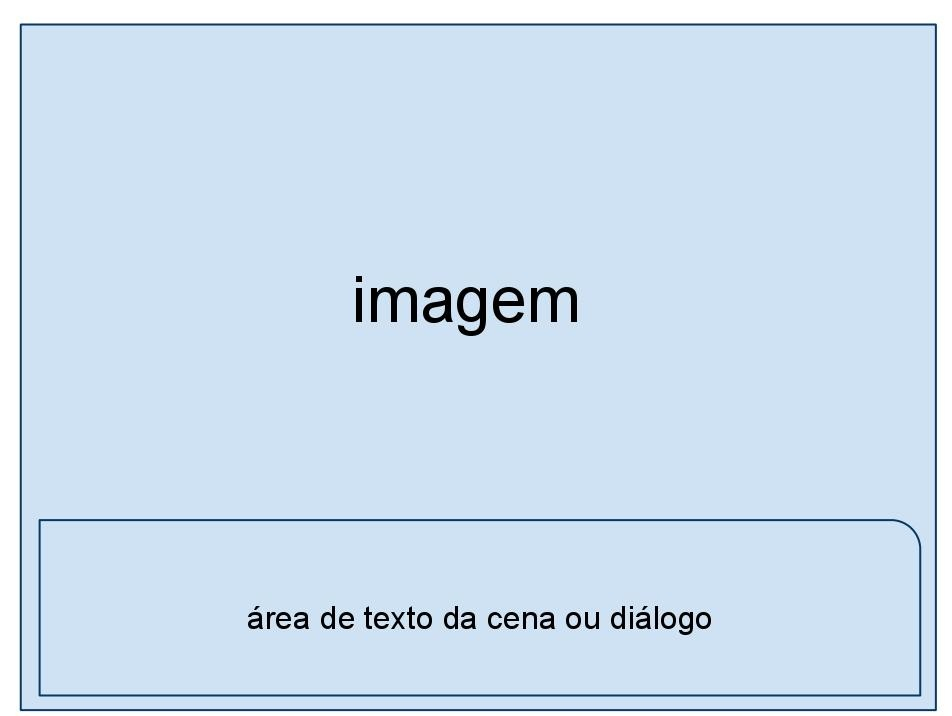
\includegraphics [width=\textwidth]{figuras/exemplo_imagem_dialogo.jpg}
\caption{Esquema de exibição de diálogo}
\label{esquemaDialogo}
\end{figure}

%
% INCLUIR FIGURA DO DIÁLOGO!
%
%

O jogador faz opção por falas digitando um número correspondente às opções apresentadas.

Já a opção de compras permite que o jogador selecione itens de uma lista e troque-os por dinheiro. É preciso que o jogador possa visualizar seu saldo então.

No reconhecimento, o jogador seleciona um de seus capangas e envia-o para observar a disposição e itens de segurança (como alarmes, câmeras e sensores de movimento) que já no lugar. note-se que é possível que isso chame a atenção de algum guarda, e aumente o nível de suspeita do capanga. Dependendo do grau de segurança do local, isso pode mesmo implicar na prisão de um do comparsas do jogador.

As opções do QG são ligeiramente distintas das demais. A opção \emph{roubo!} leva o jogador a uma sequência de telas que permitem gerenciar o roubo, escolhendo o local, os capangas que participarão, itens que cada um portará durante o troubo, e como o valor obtido será distribuído. Já \emph{conversar} leva a um diálogo com um dos capangas, que pode ser escolhido por um menu. Por fim, a opção \emph{inventário} permite observar os itens de que se dispõe, assim como com qual dos capangas ele está.

É apropriado um pouco mais de detalhe sobre o que acontece quando se inicia um roubo. A chance de sucesso de um roubo é função da habilidade dos integrantes da equipe, dos itens que possuem, da qualidade do último reconhecimento feito do local,  e do nível da segurança do alvo do roubo. Antes de confirmar o roubo, ao jogador é apresentada uma estimativa de sucesso, baseada nas informações que ele dispõe sobre o local\footnote{Essa estimativa não é necessariamente precisa, já que à princípio o jogador não sabe o grau de segurança do lugar e, também há a possibilidade de o reconhecimento efetuado ter deixado não ter identificado todos os itens de segurança.}.A execução de cada roubo recebe uma nota entre zero e dez. Notas acima de cinco indicam um roubo bem sucedido, e quanto maior a nota, maiores dividendos obtidos com ele. Por outro lado, roubos que obtenham notas abaixo de cinco representam tentativas frustradas, e o jogador será penalizado, quer tendo um de seus capangas preso, quer perdendo algum dos itens durante a fuga da equipe. De todo modo, a segurança de um lugar que tenha sido roubado é reforçada.

\section{Controles}
Praticamente todo o jogo é baseado no conceito de point-and-click, ou seja, a grande maioria dos controles é feita através do mouse. Exceto durante diálogos quando forem apresentadas diversas opções de fala ao jogador, este selecionará uma fala através do teclado, onde cada fala será representada por um número.

\section{Variações de jogo}
Existem diversas maneiras como um roubo pode ser realizado, o jogador é livre para bolar seu próprio plano. A forma de arquitetar um determinado roubo é sempre a mesma, no entanto, quanto mais o jogador investigar antes da ação e quanto mais itens (pertinentes ao roubo) o jogador utilizar, maiores são as chances do roubo ser bem sucedido.

%\section{Definições}

%\section{Referências}
